\section{Implementation Progress}

\subsection{Status}
All ten planned pipeline components work end to end on real data (Table~\ref{tab:status}). The remaining
work (P7 to P10 in Table~\ref{tab:plan}) widens the evaluation rather than adding core modules.
The code is about 1{,}930 lines of Python in 18 modules, with 40 commits on GitHub at the time of writing:
\repo.

\begin{table}[t]
\centering
\caption{Implementation status per component}
\label{tab:status}
\footnotesize
\begin{tabularx}{\columnwidth}{@{}lXc@{}}
\toprule
Component & File(s) & Status\\
\midrule
Memory extraction & \texttt{memory.py} & \done\\
Static analysis + YARA & \texttt{static.py}, \texttt{rules/crypto.yar} & \done\\
Entropy regions & \texttt{crypto/entropy.py} & \done\\
Cipher ID (56 signatures) & \texttt{crypto/identify.py}, \texttt{signatures.py} & \done\\
RSA extraction + 6 tests & \texttt{crypto/rsa\_weak.py} & \done\\
Credentials & \texttt{credentials.py} & \done\\
Network / TLS & \texttt{network.py} & \done\\
SQLite store & \texttt{store.py} & \done\\
Rule + LLM report & \texttt{report.py} & \done\\
Defences (D1 to D4) & \texttt{defences.py} & \done\\
Red-team harness & \texttt{redteam.py} & \done\\
Dashboard & \texttt{dashboard.py}, \texttt{dashboard/} & \done\\
Linux/macOS memory stage & n/a & later\\
\bottomrule
\end{tabularx}
\end{table}

\subsection{Usage}
The command-line interface exposes each part separately, which also makes the demo reproducible:
\begin{verbatim}
python -m triageguard analyze <dump> --pcap <p>
python -m triageguard crypto <any file>
python -m triageguard report <db> --out r.md
python -m triageguard redteam [--dry-run]
python -m triageguard dashboard
pytest -q
\end{verbatim}

\subsection{Problems found on real data and their fixes}
The synthetic sample was too clean. The first run on the Windows~11 image produced 689 findings and a
risk of 100. Each fix below came from reading real output; after them the same image gives 80 findings and
a risk of 55.

\begin{table}[t]
\centering
\caption{Bugs and tuning driven by real dumps}
\label{tab:bugs}
\footnotesize
\begin{tabularx}{\columnwidth}{@{}XX@{}}
\toprule
Problem on real data & Fix\\
\midrule
pyshark crashed on Python 3.14 (no event loop) & create one before opening the capture\\
a truncated PEM block aborted the run & skip damaged fragments\\
\texttt{netscan} empty on Win11 24H2 & fall back to \texttt{netstat} (52 connections)\\
636 RSA keys from the certificate store & corrupt moduli excluded, clean keys summarised, size issues graded low\\
Defender JIT memory flagged as injection & grade each region; known JIT and zeroed regions low\\
risk stuck at 100 & cap points per severity\\
antivirus blocked reading extracted malware (Win10) & record as a high finding and continue\\
same code in 5 processes (Win7) & treat as system-wide component (medium)\\
LLM report cut off before its risk score (Win7) & detect truncation; rerun with low reasoning effort\\
\bottomrule
\end{tabularx}
\end{table}

\subsection{Dashboard}
Fig.~\ref{fig:dash} shows the offline dashboard used in the demo. Selecting a dump updates the overview,
cryptography, findings and report views; report citations are links to the cited finding.

\begin{figure}[t]
\centering
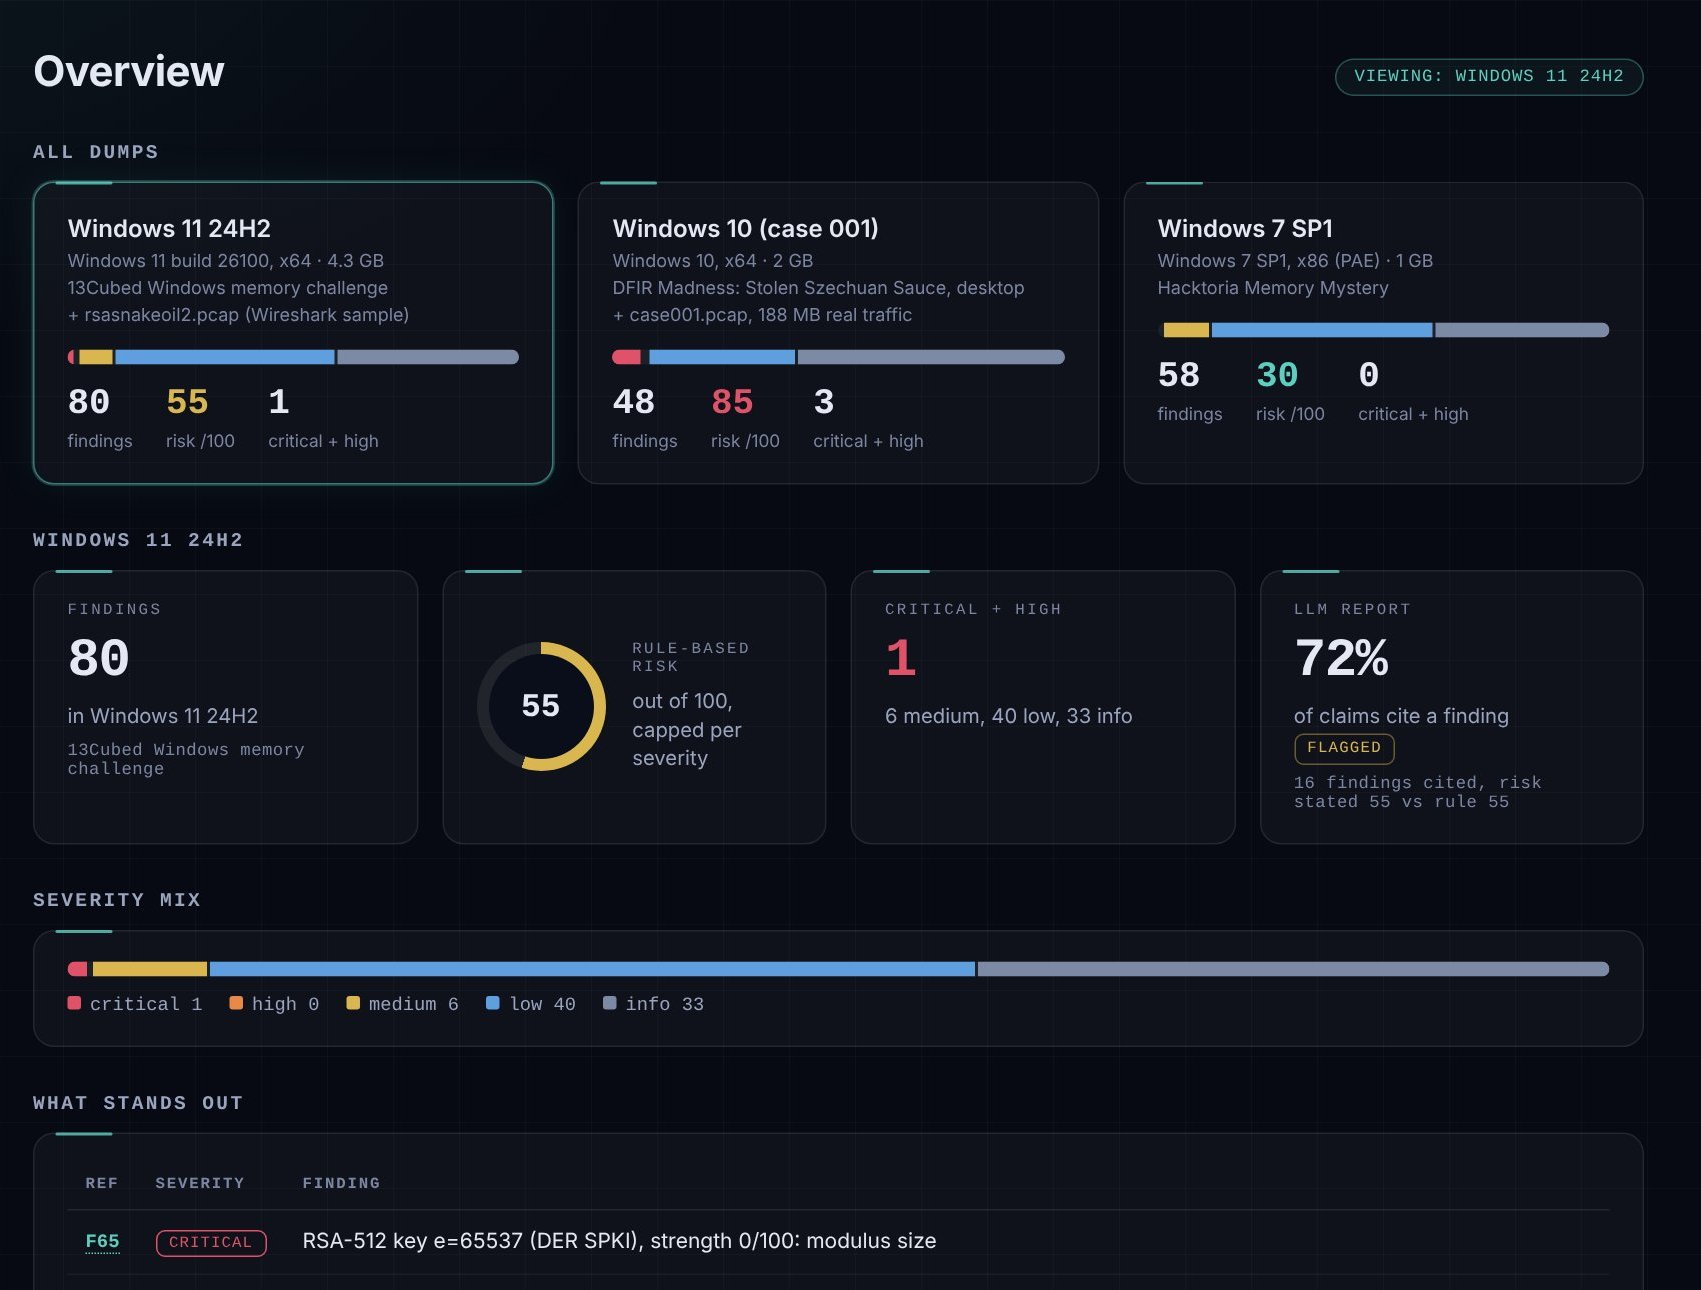
\includegraphics[width=\columnwidth]{figures/dash_overview.jpg}
\caption{Dashboard overview: three dumps, risk gauge, severity mix and the LLM report's citation coverage.}
\label{fig:dash}
\end{figure}
